\documentclass{article}

\usepackage{authblk}
\usepackage{graphicx}
\usepackage[utf8]{inputenc}
\usepackage[round]{natbib}

\bibliographystyle{copernicus}

\title{Climate uncertainty as an integral part of IAMs}
\author[1,3]{Chris Smith}
\author[2,3]{Alaa Al Khourdajie}
\author[4]{Pu Yang}
\author[5]{Doris Folini}
\affil[1]{University of Leeds, UK}
\affil[2]{Imperial College London, UK}
\affil[3]{International Institute for Applied Systems Analysis, Austria}
\affil[4]{University College London, UK}
\affil[5]{ETH Zürich, Switzerland}
\date{8 July 2022}

\begin{document}

\maketitle

\section*{Summary}

As a proof of concept, we use a simple cost-benefit integrated assessment model (DICE) coupled to a calibrated, constrained climate emulator used in the IPCC Sixth Assessment Report (FaIR) to show that inclusion of climate response and its uncertainty to emissions pathways as an integral part of IAMs is important. Without modifying the underlying economic assumptions, climate uncertainty alone permits a wide range of optimal-utility emissions trajectories that range from 4 to 41 GtCO$_2$ yr$^{-1}$ in 2100, and a social cost of carbon in 2020 of \$11 to \$35 per ton CO$_2$ (both 5-95\% ranges). 

\section*{Abstract}

Process-based integrated assessment models (IAMs) such as MESSAGE-ix and REMIND provide emissions pathways for climate emulators; a large number of these are assessed in the IPCC Working Group 3 report \citep{Kikstra2022,Riahi2022}. Climate assessment via emulators is the last step of a process chain that starts with exogenous inputs of population, urbanisation, education and GDP storylines provided by the shared socioeconomic pathways. The IAM is the energy-economy model sitting in between, solving an optimisation problem that (for example) maximises utility given these exogenous boundary conditions, subject to constraints surrounding technological deployment. In the real world, energy supply, energy demand and human decision making is likely to be a function of climate change, as is economic development with consequential effects on climate damages that lowers GDP growth \citep{Rising2022}. Some process-based IAMs are able to consider climate impacts on the energy-economic system, but as far as climate is implicitly used as a constraint in IAM scenarios it is limited to solving for a total remaining carbon budget \citep{Riahi2022} or year-2100 radiative forcing target \citep{ONeill2016}. The former relies upon the linearity and time-independence of warming with cumulative CO$_2$ emissions, and the latter relies on post-hoc assessments of emissions pathways, limited to verifying that the scenario has approximately the target forcing \citep{Gidden2019}. 

Neither of these approximate implicit climate constraints take into account how climate uncertainty could affect the optimal solution of an IAM-derived scenario. Despite recent advances, large uncertainties still exist in assessments of aerosol radiative forcing \citep{Bellouin2020}, climate sensitivity \citep{Sherwood2020}, the transient response to cumulative CO$_2$ emissions \citep{Canadell2021} and zero emissions commitment \citep{Lee2021}. The first two uncertainties strongly influence future warming \citep{Smith2019}, and the latter two define the remaining carbon budget \citep{Rogelj2019}. In reality, adaptation and mitigation effort is not likely to be independent of climate dynamics. If it turns out that climate sensitivity is high and climate is warming faster than expected, mitigation action may be ramped up in order to avoid even higher levels of warming \citep{Folini2022}.

We use a simple cost-benefit IAM, the Dynamic Integrated model of Climate and the Economy (DICE2016R; \citet{Nordhaus2017,Nordhaus2018}), as a proof of concept to show that climate uncertainty is critically important on the emissions projections, temperature, and social cost of carbon in so-called ``optimal'' pathways that maximise utility. DICE is a global model and does not include sectoral assumptions, and is structurally much simpler than processed-based IAMs, but does include a climate damage function that reduces consumption and hence utility, and so does include a climate-economy feedback that the SSP framework does not consider. DICE's simplicity also permits large ensembles given its short run time, in common with the climate emulators typically used to assess IAM emissions scenarios.

It has been noted by several authors \citep{Folini2022,Dietz2021,Gasser2021} that the climate emulator component of the DICE2016R model, in its default calibration, does not adequately reproduce results from Earth System models. Here we replace the climate component of DICE with FaIR v1.6.2 \citep{Millar2017,Smith2018,Leach2021}, specifically the setup calibrated to the latest generation of Earth System models and constrained to observations which was used to assess IAM pathways in the IPCC's Sixth Assessment Working Group 3 report \citep{Riahi2022,Kikstra2022,Byers2022,IPCC2022WG3}. Using this calibrated, constrained probabilistic calibration of FaIR \citep{Smith2021}, we run 2237 ensemble members in DICE, systematically varying the carbon cycle feedbacks, climate response (including climate sensitivity), non-CO$_2$ radiative forcing uncertainty assuming an SSP2-4.5 non-CO$_2$ forcing pathway, and observational uncertainty on near-present-day (2015) warming. The default configuration of the DICE2016R economic model is unchanged.

%Constraints on the FaIR ensemble include reproducing observed historical warming from 1850-2019 to a root-mean-squared error of less than 0.135°C, and close correspondence with distributions from IPCC assessments of 1995-2014 warming relative to 1850-1900, atmospheric CO$_2$ concentrations in 2014; aerosol radiative forcing in 2005-2014; equilibriium climate sensitivity; transient climate repsonse; transient climate response to CO$_2$ emissions; and future warming projections for SSP scenarios (Forster et al. 2021; Smith et al. 2021).

\begin{figure}[!t]
\centering
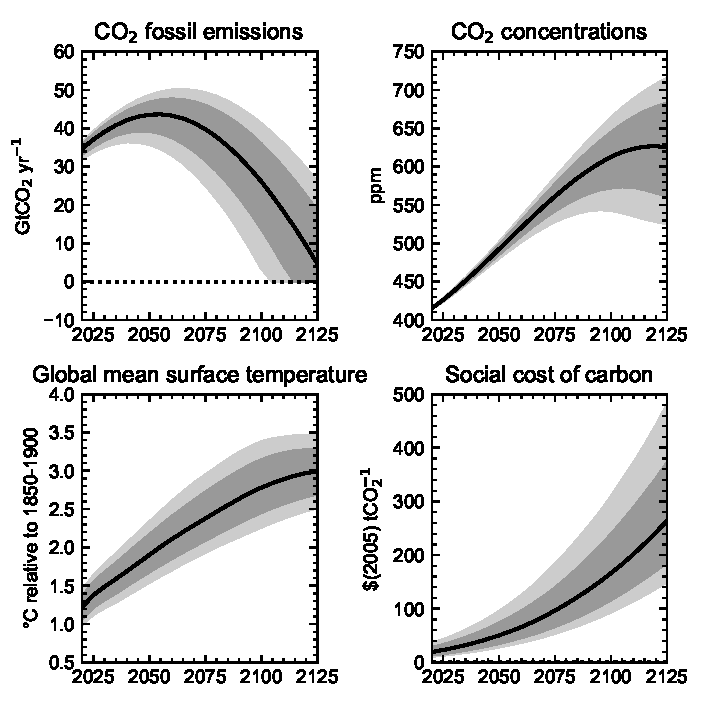
\includegraphics[width=12cm]{../../figures/climate_projections.pdf}
\caption{Projections of (a) fossil fuel CO$_2$ emissions; (b) atmospheric CO$_2$ concentrations; (c) global mean temperature projections; (d) social cost of carbon using the constrained, calibrated probabilistic ensemble of FaIR from the IPCC Sixth Assessment Report coupled to the economic model of DICE. Light shaded bands show 5-95\% range; dark shaded range show 16-84\% range; black lines show ensemble medians.}
\label{fig:projections}
\end{figure}

We show that resulting optimal emissions pathways consistent with maximisation of utility in DICE vary substantially (fig. \ref{fig:projections}a), showing a range of compatible CO$_2$ fossil fuel emissions in the range of 4 to 41 GtCO$_2$ yr$^{-1}$ in 2100 (similar spread, though slightly higher than, \citet{Folini2022}). Variation in the emissions pathways coupled with varying strengths of carbon cycle feedbacks to temperature and cumulative CO$_2$ emissions (fig. \ref{fig:projections}b). This ``optimal'' pathway results in 2.8°C (2.3-3.4°C) of warming in 2100 relative to 1850--1900 (fig. \ref{fig:projections}c), though we caution that climate damages may be underestimated in DICE \citep{Dietz2015} and no policy-relevant temperature constraints have been implemented such as a commitment to limit warming well below 2°C. Finally, the social cost of carbon also shows large variability, ranging from 11 to 35 \$ tCO$_2^{-1}$ in 2020 and increasing exponentially over the next 100 years (fig. \ref{fig:projections}d). We remark that substitution of the default climate module of DICE with FaIR results in lower median warming projections and lower levels of the social cost of carbon than in the original DICE model \citep{Nordhaus2017}, the climate component of which has been shown to respond to emissions too slowly \citep{Folini2022,Gasser2021}. Radiative forcing (not shown) is 5.5 (4.6--6.2) W m$^{-2}$ in 2100, putting these pathways somewhere between RCP4.5 and RCP6.0.

This proof-of-concept can be used in scenario development, for example to address implausibility concerns about high warming scenarios such as RCP8.5 achieving continued GDP growth that outpaces increasingly severe climate damages \citep{Woodard2019}. It would also be possible to design an ensemble consistent with holding warming to well-below 2°C scenario by stipulating that 66\% of ensemble members should remain below this threshold, to conduct a sensitivity analysis to determine the main climatic factors contributing to the uncertainty in the social cost of carbon, and to combine climate uncertainty with economic assumptions, including the choice of discount rate. The long-term goal of this work is to incorporate climate feedbacks and uncertainty into process-based IAMs, and this proof of concept shows that climate uncertainty leads to considerably different conclusions based around optimality.

\bibliography{main}

\end{document}


